\documentclass[12pt]{report}
\usepackage{caption}
\usepackage{graphicx}
\usepackage{hyperref}
\hypersetup{%
    pdfborder = {0 0 0}
}
\hypersetup{
    colorlinks,
    citecolor=blue,
    filecolor=blue,
    linkcolor=blue,
    urlcolor=blue
}
\renewcommand{\familydefault}{\sfdefault}
\renewcommand{\captionfont}{\small}

\author{Bernd Porr \& Nick Bailey}
\title{Realtime embedded coding in C++ under Linux}

\begin{document}

\maketitle

\tableofcontents

\chapter{Introduction}



\begin{figure}[!hbt]
\begin{center}
\mbox{\includegraphics[width=\textwidth]{signals-timings}}
\end{center}
\caption{Dataflow and timing in low level realtime coding
\label{timing}}
\end{figure}

\section{Event based coding in the Linux userspace}

Realtime embedded coding is all about \textsl{events}.
These can be a binary signal such as somebody opening a door or
an ADC signalling that a sample is ready to be picked up.
Fig.~\ref{timing} shows the basic dataflow and how event timing is
established: devices by themselves have event signals such as ``data
ready'' or ``crash sensor has been triggered''. The Linux kernel receives
these as interrupt callbacks. However, userspace has no direct interrupt
mechanism; instead it has \textsl{blocking I/O} where a read or write operation blocks
until a kernel-side interrupt/event has happened. A blocking I/O call returning
may then be translated to callbacks between classes by waking up threads.
Data is transmitted back to the hardware via methods called ``setters'',
which change an object's attributes and potentially do other processing.

\begin{figure}[!hbt]
\begin{center}
\mbox{\includegraphics[width=\textwidth]{gettersetters}}
\end{center}
\caption{A realtime system with two C++ classes. Communication
  between classes is achieved with callbacks (not getters) for incoming events
  and setters to send out control events. The control output itself
  receives its timing from the events so that the loop is traversed
  as quickly as possible.
\label{gettersetters}}
\end{figure}
Fig.~\ref{gettersetters} shows the overall communication between C++
classes in a realtime system. This communication is done via \textbf{callbacks}
(\textsl{not} getters) and setters, where an event from a sensor
traverses according to its realtime requirements through the C++ classes via
callbacks and then back to the control output via setters. For example,
a collision sensor at a robot triggers a GPIO pin, which then triggers a
callback to issue an avoidance action which in turn then sets the
motors in reverse.

Callbacks can be seen as userspace interrupt service routines.
These must always complete immediately so that the caller does
not experience any noticeable delay. For example when a user
presses a button in a GUI the callback must be
processed without any noticeable delay which is application specific.
If processing takes
longer then a thread should be started which in turn then will
then have a callback signalling success.

In the following sections we are describing how to write event driven
code in C++. Important here is
\begin{enumerate}
\item blocking I/O and,
\item threads woken up by blocking I/O.
\end{enumerate}
Chapter~\ref{drivers} focuses on how to wrap the low
level blocking Linux I/O in a class and how to establish the
communication between classes while the chapter~\ref{threads}
describes how threads can effectively be used to trigger callbacks
with blocking I/O. Chapter~\ref{qt} then presents the event based
communication in Qt, in particular user interaction and animations.
Chapter~\ref{webserver} tackles the same issues as for Qt but for
website server communication. The final chapter~\ref{setters} then
describes how events are transmitted back from a C++ class to the user
with the help of setters.


\chapter{Writing C++ classes for userspace event processing\label{drivers}}
This chapter focuses on writing your own C++ class for event processing by
hiding away the complexity (and messy) low level C APIs and/or raw
device access. How are events translated into I/O operations? On the
hardware-side we have event signals such as data-ready signals or by
the timing of a serial or audio interface. The Linux kernel translates
this timing info into blocking I/O on the pseudo filesystem \texttt{/dev}
which means that a read operation blocks until data has arrived
or an event has happened. The task of a C++ programmer is
to hide this complexity and these quite different approaches in C++
classes which communicate via callbacks and setters with the client
classes.

\section{General recommendations on how to write C++ event processing classes}
As said above the main purpose of object oriented coding here is to
hide away the complexity of low level driver access and offer the
client a simple and safe way of connecting to the sensor. In
particular:
\begin{enumerate}
\item Setters and callbacks hand over \textsl{physical units}
  (temperature, acceleration, \ldots) or relative units but not raw
  integer values with no meaning.
\item The sensor is configured by specifying physical units (time,
  voltage, temperature) and not sensor registers. Default config parameters
  should be specified that the class can be used straight away with
  default parameters.
\item In the build system bundle classes into separate libraries so that they
  can be re-used easily.
\item The class comes with simple demo programs demonstrating how
  a client program might use it.
\end{enumerate}



\section{Callbacks between C++ classes}
Events between C++ classes are transmitted via callbacks.
There are different ways of tackling the issue of callbacks but the
most effective way is defining a method in an \textsl{interface class} as \textsl{abstract} and asking the
client class to implement it in a derived class.

The callback is part of an interface class:
\begin{verbatim}
  struct ADSCallbackInterface {
	    /**
	     * Called when a new sample is available.
	     * This needs to be implemented in a derived
	     * class by the client. Defined as abstract.
	     * \param sample Voltage from the selected channel.
	     **/
	virtual void hasADS1115Sample(float sample) = 0;
    };
\end{verbatim}
and then registering it in the main device driver class:
\begin{verbatim}
    void registerCallback(ADSCallbackInterface* ci) {
	adsCallbackInterfaces.push_back(ci);
    }
\end{verbatim}
where \texttt{adsCallbackInterfaces} is a \texttt{std::vector} of containing instances of
\texttt{ADSCallbackInterface}.

This then allows the C++ class to transmit an event to the receiving classes by looping through
the interface pointers:
\begin{verbatim}
for(auto &cb: adsCallbackInterfaces) {
    cb->hasADS1115Sample(v);
}
\end{verbatim}

See \url{https://github.com/berndporr/rpi_ads1115} for a complete example.

Note that an interface can also be defined by \texttt{std::function} but this is a lot
slower than using interfaces. The reason is that interfaces are standard C++ and the
compiler can optimise these constructs while \texttt{std::function} does a lot of trickery
behind the scenes which a compiler won't understand and thus won't be able to optimise.
The other reason why \texttt{std::function} is discouraged is the difficulty to provide
proper documentation for the function arguments and return values.

\subsection{Callback arguments}
Above the callbacks just delivered one floating point value. However,
often more than one sample or more complex data are transmitted:
\begin{itemize}
\item Complex data: do not put loads of arguments into the
  callback but define a \textsl{struct}. For example an ADC might
  deliver all 4 channels at once:
\begin{verbatim}
class ADmulti {

        struct ADCSample {
            float ch1;
            float ch2;
            float ch3;
            float ch4;
        };

        ...
        virtual void hasSample(ADCSample& sample) = 0;
        ...
};
\end{verbatim}
Depending on your application,
you might consider the values not useful individually and therefore prefer
a \texttt{std::tuple}.
\item Arrays: Use arrays which contain the length of the arrays:
  either std::array, std::vector, etc or const arrays and then
  references to these so that the callback knows the length.
  For example the LIDAR callback uses a reference to a const length
  array:
\begin{verbatim}
/**
 * Callback interface which needs to be implemented by the user.
 **/
struct DataInterface {
        virtual void newScanAvail(
                float rpm, 
                A1LidarData (&)[A1Lidar::nDistance]) = 0;
};
\end{verbatim}
Here \texttt{A1Lidar::nDistance} is a constant-expression giving the fixed array length,
and \texttt{(\&)[A1Lidar::nDistance]} a reference to a constant-length array which
containing \texttt{A1LidarData} stucts. If you're going to use types that hard to key-in
often, \texttt{typedef} them.
\end{itemize}
In terms of \textsl{memory management}:
\begin{enumerate}
\item Low sampling rate complex data structures: allocate as a local variable. It can be a simple type
  or a struct. See \texttt{dataReady()} in: \url{https://github.com/berndporr/LSM9DS1_RaspberryPi_CPP_Library/blob/master/LSM9DS1.cpp}.
\item High sampling rate buffers: allocate memory on the heap in the
  constructor or in the private section of the class as a const length
  array and pass on a \textsl{reference}. See \texttt{getData()} in
  \url{https://github.com/berndporr/rplidar_rpi}.
\end{enumerate}






\section{Low level userspace device access}
The following sections provide pointers of how to write
the C++ driver classes for different hardware protocols which then emit events via callback interfaces.

To emulate an ``interrupt'' or event in userspace we need blocking I/O which provides the timing for example
when waiting for a GPIO change, doing audio or video I/O.

Generally any userspace program talks to the kernel via pseudo files in the \texttt{/dev} or \texttt{/sys}
directories.



\subsection{Video camera capture (openCV)}
\subsubsection{Ubuntu / Debian Linux systems\label{videodesk}}
Reading from a video camera is usually done with the help of openCV which
in turn then talks to the low level C API which in turn talks to the kernel
via \texttt{/dev/video*}.
\begin{verbatim}
while(running) {
    cv::Mat cap;
    videoCapture.read(cap);
    sceneCallback->nextScene(cap);
}
\end{verbatim}
The \texttt{read(cap)} command is blocking till a new frame has
arrived which is then transmitted with the callback \texttt{nextScene}
to the client. The full code of the example camera class is here:
\url{https://github.com/berndporr/opencv-camera-callback}.


\subsubsection{Raspberry PI}
On the raspberry PI a new video stack has been implemented which talks
to the kernel via \texttt{/dev/media*}. This is incompatible with
openCV and the code in section~\ref{videodesk} won't work. The good
news is that \texttt{libcamera} already implements a callback. Instead, one just needs to register a
callback to receive the video frames. The bad news is that libcamera
is highly complex and requires a lot of additional code
(\url{https://github.com/libcamera-org/libcamera/blob/master/Documentation/guides/application-developer.rst}).
To make life easier we have written a C++ wrapper around the libcamera C++ API
which exposes a callback which delivers image frames in openCV format to
mimick the behaviour of the openCV code of the previous
section~\ref{videodesk}:
\url{https://github.com/berndporr/libcamera2opencv}.





\subsection{Audio (ALSA)}
The standard framework for audio is alsa: \url{https://github.com/alsa-project}.

ALSA is packet based with a read command
returning a chunk ("buffer") of audio and write emitting one.
There are calls to set the sample format, sample rate, buffer size
and so forth.

First, the parameters are requested and the driver can modify or
reject them:
\begin{verbatim}
/* Signed 16-bit little-endian format */
  snd_pcm_hw_params_set_format(handle, params,
                               SND_PCM_FORMAT_S16_LE);

  /* One channel (mono) */
  snd_pcm_hw_params_set_channels(handle, params, 1);

  /* 44100 bits/second sampling rate (CD quality) */
  val = 44100;
  snd_pcm_hw_params_set_rate_near(handle, params,
                                  &val, &dir);
\end{verbatim}

Then playing sound is done in an endless loop were a read()
or write() command is issued. Both are blocking so that
they guarantee event timing of audio both way.

\begin{verbatim}
 while (running) {
   if ((err = snd_pcm_readi (handle, buffer, buffer_frames)) != buffer_frames) {
     if (errCallback) errCallback->hasError();
   }
   if (sampleCallback) sampleCallback->hasData(buffer);
 }
\end{verbatim}

For a full coding example ``aplay'' and ``arecord'' are a good start.
Both can be found here:
\url{https://github.com/alsa-project}.



\subsection{Bluetooth}

Bluetooth has also blocking I/O so that one can wait for incoming packets on a socket:

\begin{verbatim}
void run() {
        doRun = 1;
        while (doRun) {
                recv(btsocket, recvbuffer, sizeof(recvbuffer), 0);
                hasData(recvbuffer);
        }
};
\end{verbatim}

Here the \texttt{recv} command blocks until new data has arrived.





\subsection{General purpose I/O (GPIO)}
GPIO pins are not just simple digital ports but they
can be used to turn non-blocking I/O into blocking I/O, or in other words: events!
SPI and I2C are only blocking for their read/write operations but they don't know
when new data is available at a sensor so one needs to connect the DATA-READY output
of a sensor to a GPIO port which then feeds into blocking I/O.

\subsubsection{libgpiod}
The GPIO (of the raspberry PI) can easily be controlled via
the \texttt{/dev} filesystem and \texttt{libgpiod}.

Use the commandline tool
\texttt{gpioinfo} to print a list of all available GPIO pins.

When you use the gpiod library you:
\begin{enumerate}
\item first choose the GPIO \textsl{chip} you want to use. Raspberry PIs 1-4
  have only one chip. The Raspberry PI 5 has 4 chips.
  Selection can be made either by number, name or pseudo-file:
\begin{verbatim}
  struct gpiod_chip *chip = 
             gpiod_chip_open_by_name("gpiochip0");
\end{verbatim}
and then,
\item select a pin on the chip:
\begin{verbatim}
  struct gpiod_line *pinRed =
             gpiod_chip_get_line(chip, 24);
\end{verbatim}
\end{enumerate}

\subsubsection{Output}
Once you have a pointer to the pin you can then set its direction, for example
as an output pin, with:
\begin{verbatim}
gpiod_line_request_output(pinRed, "example1", 0);
\end{verbatim}
and set its value with:
\begin{verbatim}
gpiod_line_set_value(pinRed, 1);
\end{verbatim}

\subsubsection{Events}
libgpiod offers all the functionality of event processing via blocking I/O!
Here, change in level from low to high or high
to low unblocks an I/O operation, awakening its underlying
thread which then one can perform a callback.

To request event processing on a pin simply
requires this single
command:
\begin{verbatim}
int ret =
   gpiod_line_request_rising_edge_events(pinSwitch, "Consumer1");
\end{verbatim}
This will turn the GPIO pin \texttt{pinSwitch} into an input pin and enable
blocking I/O on this pin.

Then start a thread where its worker contains:
\begin{verbatim}
void worker() {
    while (running) {
        constexpr struct timespec ts = { 1, 0 };
        gpiod_line_event_wait(pinSwitch, &ts);
        struct gpiod_line_event event;
        gpiod_line_event_read(pinSwitch, &event);
        event_callback();
    }
}
\end{verbatim}
The \texttt{gpiod\_line\_event\_wait} waits for a rising edge at the GPIO
pin, or for 1~second (+ 0\,ns), whichever is longer, and then unblocks.
The return value is 1 if a GPIO event occurred, 0 if timeout interval
was exceeded, and -1 in the event of an error. In production code,
you'd need to check this return value.
Then \texttt{gpiod\_line\_event\_read} transfers the
kernel event to userspace and clears it out of the kernel event queue.
It's important to do the read operation
even if the event-struct is never used. The callback is made,
and the loop repeats until another thread requests termination
by setting \verb!running! to \verb!false!.
See \url{https://github.com/berndporr/libgpiod_event_demo} for a complete example.

\subsubsection{Releasing the GPIO}
Once you are finished, release the GPIO pin with:
\begin{verbatim}
    gpiod_line_release(pinRed);
\end{verbatim}
and close the chip:
\begin{verbatim}
    gpiod_chip_close(chip);
\end{verbatim}







\subsection{SPI}
\begin{table}[!ht]
  \begin{center}
  \caption{SPI modes\label{spimodes}}
  \begin{tabular}{l|l|l|l}
    SPI Mode & 	CPOL & 	CPHA & Idle state \\
    \hline
    0& 	0&	0& 	L \\
    1& 	0&	1& 	L \\
    2& 	1&	1& 	H \\
    3& 	1&	0& 	H \\
  \end{tabular}
  \end{center}
\end{table}
SPI is a protocol which usually transmits and receives at the same
time. Its calls are blocking for the duration of receive and transmit but cannot be used for
event based processing. If an SPI device is used events should be transmitted via an additional
GPIO line. 
Even though data might not be used it needs to be matched up,
because the same clock is used to send and collect the data signal
(it is \emph{isochronous}).
So if you send 8 bytes the hardware receives 8 bytes at the same time.

Transfer to/from SPI is best managed by the low level access to \texttt{/dev}.
Open the SPI device with the standard \texttt{open()} function:
\begin{verbatim}
int fd = open( "/dev/spidev0.0", O_RDWR);
\end{verbatim}

Then set the SPI mode (see table~\ref{spimodes}):
\begin{verbatim}
int ret = ioctl(fd, SPI_IOC_WR_MODE, &mode);
\end{verbatim}
as explained, for example, here:
\url{https://www.analog.com/en/analog-dialogue/articles/introduction-to-spi-interface.html}.

Because SPI is isochronous, \texttt{read()} and \texttt{write()}
can't be used to transmit and receive data. Instead, the simultaneous
read and write is performed using an \texttt{ioctl()} to do the communication.
Populate this struct:
\begin{verbatim}
struct spi_ioc_transfer tr {
  .tx_buf = (unsigned long)tx1,
  .rx_buf = (unsigned long)rx1,
  .len = ARRAY_SIZE(tx1),
  .delay_usecs = delay,
  .speed_hz = speed,
  .bits_per_word = 8,
};
\end{verbatim}
which points to two character buffers ``tx'' and ``rx'' with the
same length\footnote{This code fragment's use of designated initialisers
officially requires C++2a, although most C++ compilers support it
when compiling with older standards. In C it's been fine for a while!}.

Reading and simultaneous writing then happens via this \texttt{ioctrl()}
function call:
\begin{verbatim}
int ret = ioctl(fd, SPI_IOC_MESSAGE(1), &tr);
\end{verbatim}

Sometimes the SPI protocol of a chip is so odd that even the raw I/O
via \texttt{/dev} won't work and you need to write your own bit
banging interface, for example done here for the ADC on the alphabot:
\url{https://github.com/berndporr/alphabot/blob/main/alphabot.cpp#L58}.
This is obviously far from ideal as it might require \texttt{usleep()}
commands so that acquisition needs to be run in a separate thread (the
alphabot indeed uses a timer callback in a separate thread).

Overall the SPI protocol is often device dependent and calls
for experimentation to get it to work. On some ADCs the SPI clock is also
the conversion clock and a longer lasting clock signal sequence is required,
making it necessary to transmit dummy bytes in addition to the payload.

As a general recommendation do not use SAR converters which use the
SPI data clock also as acquisition clock as they are often not compatible
with the standard SPI transfers via \texttt{/dev}. Use sensors or ADCs which
have their own clock signal.


\subsection{I2C}
I2C is a protocol which either receives or transmits. Its I/O operations are blocking but only
for the duration of receive or transmit. Use an additional GPIO pin for
events for example for a data-ready event.

The I2C bus has two signal lines (SDA \& SDL) which must be pulled up
by resistors. Every I2C device has an address on the bus. You can scan
a bus with \textbf{i2cdetect} (part of the i2c-tools package):
\begin{verbatim}
root@raspberrypi:/home/pi# i2cdetect -y 1
     0  1  2  3  4  5  6  7  8  9  a  b  c  d  e  f
00:                         -- -- -- -- -- -- -- -- 
10: -- -- -- -- -- -- -- -- -- -- -- -- -- -- 1e -- 
20: -- -- -- -- -- -- -- -- -- -- -- -- -- -- -- -- 
30: -- -- -- -- -- -- -- -- -- -- -- -- -- -- -- -- 
40: -- -- -- -- -- -- -- -- -- -- -- -- -- -- -- -- 
50: -- -- -- -- -- -- -- -- 58 -- -- -- -- -- -- -- 
60: -- -- -- -- -- -- -- -- -- -- -- 6b -- -- -- -- 
70: -- -- -- -- -- -- -- --                         
root@raspberrypi:/home/pi# 
\end{verbatim}
In this case there are 3 I2C devices on the I2C bus at addresses
1E, 58 and 6B and need to be specified when
accessing the I2C device.

\subsubsection{Raw \texttt{/dev/i2c} access}
I2C either transmits or receives but never at the same time so here we
can use the standard C read/write commands. However, we need to use ioctrl to tell
the kernel the I2C address:
\begin{verbatim}
char buf[2];
int file = open("/dev/i2c-2",O_RDWR);
int addr = 0x58;
ioctl(file, I2C_SLAVE, addr);
write(file, buf, 1)
read(file, buf, 2)
\end{verbatim}
where \texttt{addr} is the I2C address. Then use standard \texttt{read()}
or \texttt{write()} commands. Usually the 1st write operation tells the chip
which register to read or write to. Subsequent operations read
or write that register. For example, reading a 16~bit register:
\begin{verbatim}
unsigned 2c_readWord(uint8_t reg)
{
	uint8_t tmp[2];
	tmp[0] = reg;
	write(fd_i2c,&tmp,1);
        read(fd_i2c, tmp, 2);
        return (((unsigned)(tmp[0])) << 8) | ((unsigned)(tmp[1]));
}
\end{verbatim}
Similarly writing a 16~bit register writes 3 bytes to the I2C bus (register and the 16~bit data):
\begin{verbatim}
void i2c_writeWord(uint8_t reg, unsigned data)
{
	uint8_t tmp[3];
	tmp[0] = reg;
	tmp[1] = (char)((data & 0xff00) >> 8);
	tmp[2] = (char)(data & 0x00ff);
	write(fd_i2c,&tmp,3);
}
\end{verbatim}


\subsection{Access to hardware via special devices in \texttt{/sys}}
Some sensors are directly available via the sys filesystem in human readable format.
For example
\begin{verbatim}
cat /sys/class/thermal/thermal_zone0/temp
\end{verbatim}
gives you the temperature of the CPU.






\subsection{Accessing physical memory locations (danger!)}
Don't.
In case you really need to access registers you can
also access memory directly. This should only be used as a last resort.
For example, setting the clock for the AD converter requires
turning a GPIO pin into a clock output pin. This is not yet
supported by the drivers so we need to program registers
on the RPI.
\begin{itemize}
\item Linux uses virtual addresses so that a pointer won't
point to a physical memory location. It points to three page
tables with an offset.
\item Special device \texttt{/dev/mem} allows access to physical
memory.
\item The command \textbf{mmap} provides a pointer to a physical
address by opening \texttt{/dev/mem}.
\item Example:
\begin{verbatim}
int *addr;
if ((fd = open("/dev/mem", O_RDWR|O_SYNC)) < 0 ) {
    printf("Error opening file. \n");
    close(fd);
    return (-1);
}
addr = (int *)mmap(0, num*STRUCT_PAGE_SIZE, PROT_READ, MAP_PRIVATE,
            fd, 0x0000620000000000);
printf("addr: %p \n",addr);
printf("addr: %d \n",*addr);
\end{verbatim}
\item Use this with care! It's dangerous if not used properly.
\end{itemize}


\section{Kernel driver programming}
You can also create your own \texttt{/dev/mydevice} in the \texttt{/dev} filesystem
by writing a kernel driver and a matching userspace library. For
example the USB mouse has a driver in kernel space and translates
the raw data from the mouse into coordinates. However,
this is beyond the scope of this handout. If you want to embark
on this adventure then the best approach is to
find a kernel driver which does approximately what you want and
modify it for your purposes.


\section{Conclusion}
The communication between C++ classes is achieved via
callbacks and setters. The event from the sensor traverses
the C++ classes via callbacks and then back to the control
output via setters.

From the sections above it's clear that Linux user-space low level
device access is complex, even without taking into account the
complexity of contemporary chips which have often a multitude of
registers and pages of documentation. Your task is to hide away
all this (scary) complexity in a C++ class and offer the client
an easy-to-understand interface.





\chapter{Threads\label{threads}}

\section{Introduction}
In realtime systems threads have two distinct functions:
\begin{enumerate}
\item Loops with blocking I/O
  to establish \textbf{precise timing} for callbacks.
\item \textbf{Asynchronous execution} of time-consuming tasks
  with a callback after the task has completed.
\end{enumerate}


\section{Processes and Threads}
Processes are different programs which seem to be running at the same
time. A small embedded system may only have a single CPU core,
so this this is achieved by the operating system switching
approximately every 10ms from one process to the next so it feels as
if they are running concurrently. A thread is a lightweight
process. A process may have  multiple threads which share the same
address-space and are all started from
within the parent process. As with processes, the threads seem to be
running at the same time. When a thread is started it runs
simultaneously with the main process which created it.

\section{Thread and worker}
A thread is just a \textsl{wrapper} for the actual method
which is running independently. The method being run in the thread
is often called a \textsl{worker}.

\subsection{Creating threads}
In C++ a worker is a method within
a class:
\begin{verbatim}
uthread = std::thread(&MyClassWithAThread::run, this);
\end{verbatim}
where \texttt{MyClassWithAThread} is a class containing the function ``run'':
\begin{verbatim}
class MyClassWithAThread {
        void run() {
                // ... hard work is done here
                doCallback(result); // hand the result over
        }
}
\end{verbatim}
Note that the \& signifies a functor, a method prototype.
Instead of using functors you can also use a lambda function
to call a method in the instance:
\begin{verbatim}
uthread = std::thread([this](){run();});
\end{verbatim}


\subsection{Lifetime of a thread}
Threads terminate simply once the worker has finished its job.
To tell the client that a thread has finished you can use a
\textsl{callback} to trigger an event.

Sometimes it's important to wait for the termination of the thread,
for example when your whole program is terminating or when
you stop an endless loop in a thread. To wait for the termination
of the thread use the ``join()'' method:
\begin{verbatim}
        void stop() {
                uthread.join();
        }
\end{verbatim}
In a realtime system \texttt{join} is most likely only needed when shutting down the program.


\subsection{Running/stopping workers with endless loops}
Threads with endless loops are often used in conjunction with blocking
I/O which provide the timing:
\begin{verbatim}
void run() {
       running = true;
       while (running) {
              read(buffer); // blocking
              doCallback(buffer); // hand data to client
       }
}
\end{verbatim}
Note the flag \texttt{running} which is controlled by the main program and is set to zero to terminate
the thread:
\begin{verbatim}
        void stop() {
                running = false; // <----- HERE!!
                uthread.join();
        }
\end{verbatim}
Note that \texttt{join()} is a blocking operation and needs to be used with care not to
lock up the main program. You probably only need it when your program is terminating.
See \url{https://github.com/berndporr/rpi_AD7705_daq} for an example.

If your program creates and joins several threads while executing,
with care you might be able to design your program to allow an
end-of-life thread to carry on
tidying up in the background after you stop it by setting \texttt{running = false;}.
In this case only need execute \texttt{join()} to be sure that
the thread has finished. Joining a terminated thread is OK
(the call just returns immediately)
but you absolutely must not join a thread more than once,
nor delete a thread until you've joined it.


\subsection{Timing within threads}
Threads are perfect to create timing without using \texttt{sleep} commands
with the help of \textsl{blocking I/O}. 
Blocking I/O puts a thread
to sleep and is woken up after new data has arrived or has been
written to a device. Blocking I/O won't consume any CPU power
and is perfect to tell the kernel that it can execute other threads
in the meantime.


\subsubsection{Timing with blocking I/O}
Blocking I/O (read, write, etc) \textsl{is by far the best approach} to time
the data coming in because the thread goes to sleep when it's waiting for
I/O but wakes up very quickly after new data has arrived.

In this example the blocking \texttt{read} command creates
the timing of the callback:
\begin{verbatim}
void run() {
       running = 1;
       while (running) {
              read(buffer); // blocking
              doCallback(buffer); // hand data to client
       }
}
\end{verbatim}
If the I/O is non-blocking or if you are making blocking I/O non-blocking with:
\begin{verbatim}
int flags = fcntl(fd, F_GETFL, 0);
fcntl(fd, F_SETFL, flags | O_NONBLOCK);
\end{verbatim}
you can then use \texttt{select()} which blocks on the file descriptor:
\begin{verbatim}
FD_ZERO(&rdset);
FD_SET(fd,&rdset);
struct timeval timeout;
timeout.tv_sec = 0;
timeout.tv_usec = 500000;
int ret = select(fd+1,&rdset,NULL,NULL,&timeout);
if (ret < 0) return ret;
// non-blocking I/O read
ret = read(fd,buffer,bytes_per_sample * n_chan);
\end{verbatim}
which has the advantage that it has a timeout so that
you can create both error and data
callbacks. Even if the I/O is blocking using select or poll
has the advantage that these commands have timeouts while
the read and write commands would block forever. This is also
the recommended approach for libgpiod where the \texttt{gpiod\_line\_event\_wait}
is not needed because \texttt{gpiod\_line\_event\_read} is blocking
but would block indefinitely.


\section{Timing with Linux timers}
If no timing info from the sensor is available
one can use a timer as a last resort. Under Linux reliable timing
can be again created with the help of blocking I/O
and threads. Here, a
special file descriptor receives information when a timer
has fired first and at which intervals
after:
\begin{verbatim}
fd = timerfd_create(CLOCK_MONOTONIC, 0);
its.it_value.tv_sec = millisecs / 1000;
its.it_value.tv_nsec = (millisecs % 1000) * 1000000;
its.it_interval.tv_sec = millisecs / 1000;
its.it_interval.tv_nsec = (millisecs % 1000) * 1000000;
if (timerfd_settime(fd, 0, &its, NULL) == -1)
  throw("Could not start timer");
\end{verbatim}
This file descriptor is then used
in a loop with a blocking \texttt{read} command which then
wakes up at the specified intervals:
\begin{verbatim}
running = true;
while (running) {
  uint64_t exp;
  read(fd, &exp, sizeof(uint64_t));
  timerEvent();
}
\end{verbatim}
where \texttt{timerEvent} is as usual the callback which is
called at the specified intervals.

However, generally it's \textsl{not recommended}
to use timers for anything which needs to be sampled at high temporal
precision, for
example ADC converters or sensors with sampling rates higher than a
few Hz.

\section{Conclusion}
Threads play a central role in real-time coding as,
together with blocking I/O, they establish
the callback interfaces. Every event handler
runs in a separate thread.

Callbacks are also used to signal the termination of
threads, which shows again the close relationship between threads
and callbacks.



\chapter{Realtime/event processing within the Graphical User Interface Qt\label{qt}}

\section{Introduction}
\textbf{Qt} is a cross-platform windows development environment for
Linux, Windows and Mac. Such graphical user interfaces have realtime
requirements because, for example, pressing a button should trigger an
instant response by the application so that the user thinks this has
been instantaneous. QT also works with callbacks as introduced above
but they are wrapped in a QT-specific signal/slot concept.

Elements in Qt are \textsl{Widgets} which can contain anything form
plots, buttons or text fields. They are classes. You can define your
own widgets or use ready-made ones. Realtime communication within QT
happens between widgets where then one widget calls another widget,
for example a button the calls the main window if a button press has
happened.

\begin{figure}[!hbt]
\begin{center}
\mbox{\includegraphics[width=0.5\textwidth]{qwtex}}
\end{center}
\caption{QT example layout
\label{qwtex}}
\end{figure}

The arrangements of widgets on the screen is managed by
layouts. There are different ways of declaring layout in Qt. One is
using a markup language which then has matching classes;
another is creating to use only C++ classes.
We show how to organise the layout using the second method.
This avoids having the learn an additional language and is
consistent with the general  trend to use code to declare the layout
in this and other frameworks (\textbf{SwiftUI}, for example).

This is an example how widgets are organised into
nested vertical and horizontal layouts (see Fig.~\ref{qwtex}
for the result).
\begin{verbatim}
// create 3 widgets
button = new QPushButton;
thermo = new QwtThermo; 
plot = new QwtPlot;

// vertical layout
vLayout = new QVBoxLayout;
vLayout->addWidget(button);
vLayout->addWidget(thermo);

// horizontal layout
hLayout = new QHBoxLayout;
hLayout->addLayout(vLayout);
hLayout->addWidget(plot);

// main layout
setLayout(hLayout);
\end{verbatim}


\section{Callbacks in Qt}
\subsection{Events from widgets}
In contrast to our low level callback mechanism using interfaces, Qt rather
directly calls methods in classes. The problem is that function pointers
cannot be directly used as a class has instance pointers to its local
data. So a method of a class needs to be combined with the instance
pointer. The Qt method ``connect'' does exactly that:
\begin{verbatim}
connect(button, &QPushButton::clicked,
        this, &Window::reset);
\end{verbatim}
The QPushButton instance \texttt{button} has a method called \texttt{clicked()} which is
called whenever the user clicks on the button. This is then forwarded to the
method \texttt{reset()} in the application Widget.


\subsection{Plotting realtime data arriving via a callback}
The general idea is to store the real-time samples from a callback in a
buffer and trigger a screen refresh at a lower rate. For example, we may
choose to replot the samples in the buffer every
40~ms because that fast enough for the user, whereas plotting the
whole buffer every sample would be too CPU-intensive.

A callback \texttt{addSample()} is called in real-time whenever
a sample has arrived:
%should probably change memmove to std::move or whatever
\begin{verbatim}
void Window::addSample( float v ) {
    // add the new input to the plot
    std::move( yData, yData + plotDataSize - 1, yData+1 );
    yData[0] = v;
}
\end{verbatim}
which stores the sample \texttt{v} in the shift buffer \texttt{yData}.

Then the screen refresh (which is slow) is done at
a lower and unreliable rate:
\begin{verbatim}
void Window::timerEvent( QTimerEvent * )
{
    curve->setSamples(xData, yData, plotDataSize);
    plot->replot();
    thermo->setValue( yData[0] );
    update();
}
\end{verbatim}

\texttt{update()} in the timer event-handler generates a
paint event and Qt then invokes the repaint
handler ``as soon as possible'' (which is to say, not in real-time) to repaint
the canvas of the widget:
\begin{verbatim}
void ScopeWindow::paintEvent(QPaintEvent *) {
        QPainter paint( this );

        paint.drawLine( ... )
}
\end{verbatim}

Note that neither the timer nor the \texttt{update()} function
is called in a reliable way but whenever Qt chooses to do it.
So Qt timers cannot be used to sample data but should
only be used for screen refresh and other non-time-critical
reasons.

\section{Conclusion}
Events in Qt are generated by user interaction, for example a button
press or moving the mouse. As before Qt provides a callback mechanism
via the \texttt{connect()} method. Callbacks from Qt timers may be used for
animations but must not be used for real-time events as Qt timers won't
guarantee a reliable timing.

\chapter{Realtime publisher-subscriber communication with DDS}

\begin{figure}[h]
\begin{center}
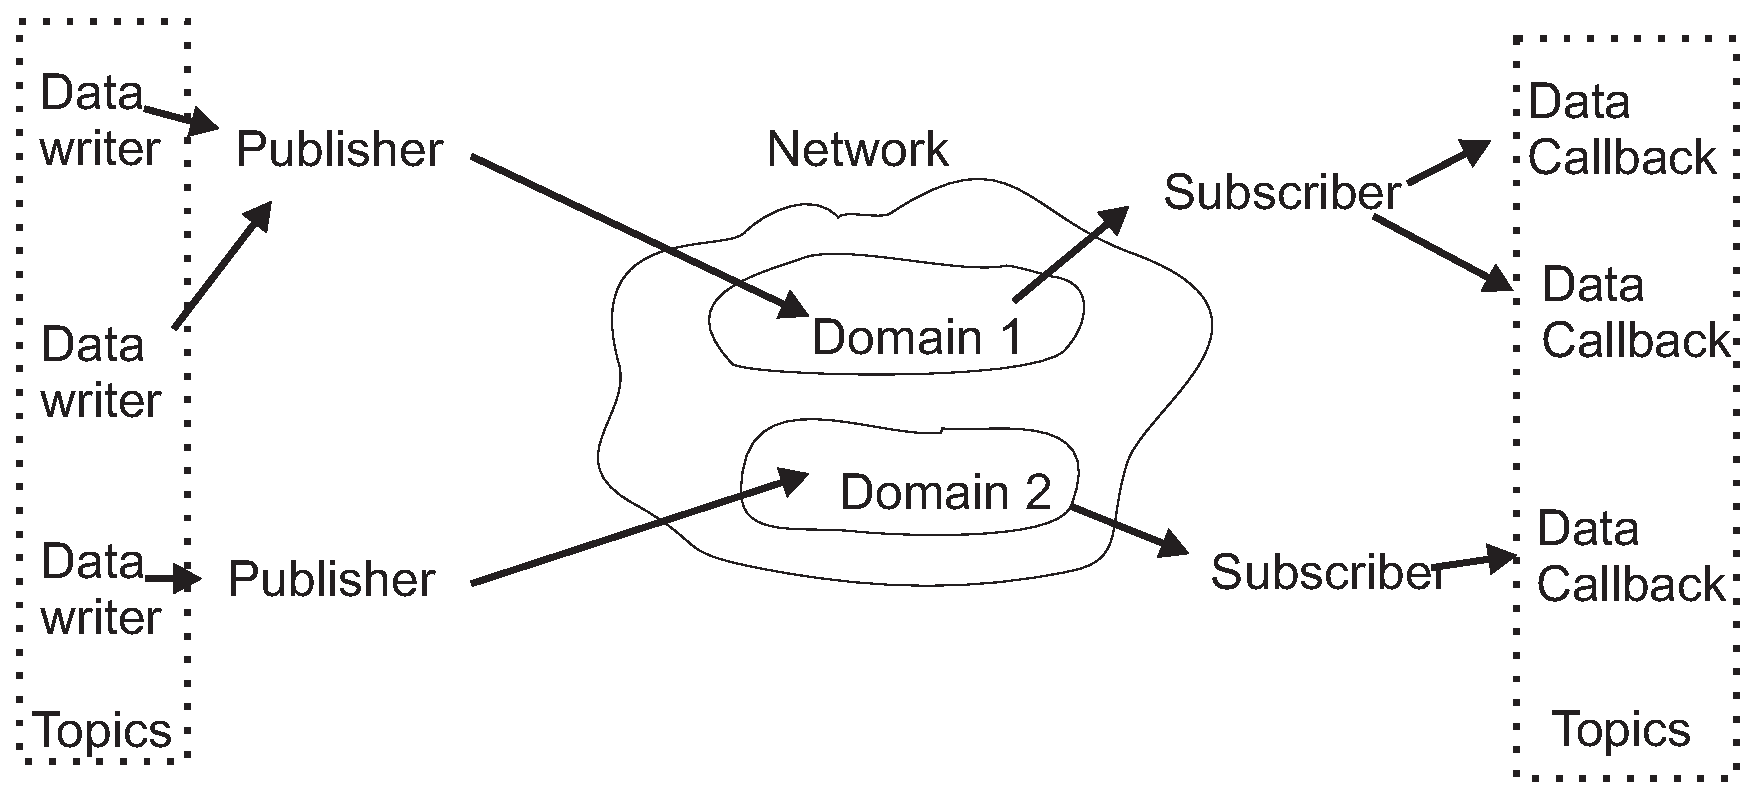
\includegraphics[width=\linewidth]{fastdds1}
\end{center}
\caption{FastDDS.\label{dds1}}
\end{figure}

So far communication has only been between classes within the same
program on the same computer. However, often data needs to be
transmitted in realtime over a network. The Data Distribution Service
(DDS) is a middleware protocol and API which has been developed to
provide reliable and low-latency publisher-subscriber communication
(see Fig.~\ref{dds1}): a publisher sends a message (here a
C++ \texttt{struct}) through a communcation channel which is called a ``topic''.
The subscriber receives messages from all the topics to which
it has subscribed, and then triggers callbacks
delivering those messages.  We focus on fastDDS which uses the
RTPS (Real Time Publish Subscribe) protocol. It offers plug and play
connectivity which won't require to specify IP addresses in a local
networks so that applications are automatically discovered. fastDDS is
now the standard middleware of ROS2, the popular robotic operating
system.

Here are the steps how to use fastDDS. A complete demo application is here: \url{https://github.com/berndporr/fastdds_demo}.

\section{Essential classes and their r\^oles}

\begin{description}
 \item[Domain] refers to a collection of actors which publish and/or subscribe to topics.
 \item[DomainParticipant] is a factory class for publishers, subscribers and topics.
 \item[Topic] means a category of messages passed between actors in the domain.
  It's the method by which a participant which receives messages may filter output
  only those that are relevant.
 \item[Publisher] participants send messages to every other participant
  which is listening for information on a given topic.
 \item[Subscriber] participants receieve messages on the topic(s) wo whcih they have
  subscribed.
\end{description}

\section{Define the data structure}

The idea with fastDDS is to specify a data structure as a C++ style
\texttt{struct} which is then converted into header and cpp files.
For example the template \texttt{HelloWorldMsg.idl}:
\begin{verbatim}
struct HelloWorldMsg
{
    unsigned long index;
    string message;
};
\end{verbatim}
contains an unsigned long int and a C++ string. This template file is then
converted to C++ header and cpp files with the helper:
\begin{verbatim}
fastddsgen HelloWorldMsg.idl
\end{verbatim}
which of course should be automated by your cmake build system.

\section{Publisher}
The Publisher wants to be able to send messages to every object that is
subscribed to its topic. It has to do three things to achieve this:
\begin{enumerate}
 \item Create a topic to which interested objects can subscribe;
 \item Create a \texttt{Publisher} which is a factory class to create any required
  writers, callback handers etc.; and
 \item Use that Publisher to create a \texttt{DataWriter} that actually
  sends messages on a particular topic.
\end{enumerate}

\subsection{Creating a Topic}

\texttt{Participant.create\_topic} is used to associate the topic with the
data structure which will be passed to that topic's subscribers.
The example program calls it like this:
\begin{verbatim}
topic_ = participant_->create_topic("HelloWorldTopic",
                                    "HelloWorldMsg",
                                    TOPIC_QOS_DEFAULT);
\end{verbatim}

\subsection{Creating a Publisher and a Writer}

Message senders and receivers  are created by a factory class, \texttt{Publisher}.
An instance of this class is required before any writers can be created.
The \texttt{Participant} can build Publishers for us using its \texttt{create\_datawriter}
method. In the example program, it looks like this:
\begin{verbatim}
publisher_ = participant_->create_publisher(PUBLISHER_QOS_DEFAULT,
                                            nullptr);
\end{verbatim}
and with that Publisher, we can create a \texttt{DataWriter}
\begin{verbatim}
writer_ = publisher_->create_datawriter(topic_,
                                        DATAWRITER_QOS_DEFAULT,
                                        &listener_);
\end{verbatim}

\subsection{Specifying the Writer's callback function}

\texttt{listener\_}, the third argument to the \texttt{create\_datawriter} method
above, is an object implementing the callback interface
spefied by the \texttt{DataWriterListener} class, specifically,
the \texttt{on\_publication\_matched} method. In the example,
the private class \texttt{PubListener} provides this functionality.
When a subscriber registers to receive messages on the topic, this is the object
which will be informed. As this is a minimalistic example, all that
\texttt{listener\_} does is to maintain a thread-safe (``atomic'') integer
which counts the number of subscribers as they connect and disconnect,
and prints messages to the console as they do so. Refer to the
\href{https://github.com/berndporr/fastdds_demo/blob/main/HelloWorldPublisher.cpp#L50}{source code} in the example to see how it works.

\subsection{Sending messages}

Having packaged this all in a class we can finally implement the method
which publishes a message. The code in the example sends the
\texttt{HelloWorldMsg} referenced by \texttt{hello} if any listners are
subscribed. If there is none, it immediately returns false; otherwise
it sends the message then returns true.

\begin{verbatim}
class HelloWorldPublisher
{
    // ... the initialisation decribed above ... then
    
    //!Send a publication
    bool publish(HelloWorldMsg& hello)
    {
        if (listener_.matched_ > 0)
        {
            writer_->write(&hello);
            return true;
        }
        return false;
    }
}
\end{verbatim}


\section{Subscriber}
The program which wants to receive data on a particular topic needs
to subscribe to that topic. The process of creating
a subscriber is similar to creating a publisher.:

\begin{enumerate}
 \item Create the participant that will interact with the topic;
 \item Register the data type which the topic uses for its messages;
 \item Ask the participant to create a subscriber to that topic;
 \item Register the callback by creating a \texttt{DataReader} which
  implements the \texttt{DataReaderListener} interface.
\end{enumerate}

\subsection{Implementation}
The relevant code from the example which sets up the infrastructure reads
very similarly to the publisher, except that of course the participant is used
to create subscriber rather than a writer:
\begin{verbatim}
topic_ = participant_->create_topic("HelloWorldTopic",
                                    "HelloWorldMsg",
                                    TOPIC_QOS_DEFAULT);
subscriber_ = participant_->create_subscriber(SUBSCRIBER_QOS_DEFAULT,
                                              nullptr);
reader_ = subscriber_->create_datareader(topic_,
                                         DATAREADER_QOS_DEFAULT,
                                         &listener_);
\end{verbatim}

\subsection{Receiving data}
\texttt{listener\_} in the publishing application was a callback object which was
called whenever a subscriber joined or left the topic. In the subscribing application
it is a callback object which receives data on the topic from a writer
whenever any becomes available. It does this by having its
\texttt{on\_data\_available} method called. This method will
invoke the Reader's \texttt{take\_next\_sample} method to acquire the
incoming message data and information, and processes it
however the receiving program requires. In the example we just print it out.
\begin{verbatim}
class SubListener : public DataReaderListener {
public:
// callback
void on_data_available(DataReader* reader) override {
  SampleInfo info;
  HelloWorldMsg hello;
  if (reader->take_next_sample(&hello, &info) == ReturnCode_t::RETCODE_OK) {
    if (info.valid_data) {
      std::cout << "Message: " << hello.message()
                               << " with index: " << hello.index()
                               << " RECEIVED." << std::endl;
    }
  }
}
\end{verbatim}

\chapter{Realtime web server/client communication\label{webserver}}

\section{Introduction}

There is a wide diversity of Web server / client applications
ranging from shopping baskets on vendor sites to social
media.

Generally it's easy to create dynamic content (see PHP or nodejs) and this is well
documented. However, feeding realtime data from C++ to a web page or
realtime button presses back to C++ is a bit more difficult.

It's important to recognise where \textsl{events} are generated: it is
always the client (web browser or mobile app) which triggers an event,
be it sending data over to the server or requesting data. It's
always initiated by the client.

\section{REST}
The interface between a web client (browser or phone app) is usually
implemented as a Representational State Transfer Architectural (REST)
API by communicating via an URL on a web server. The requirements
for this API are very general and won't define the actual data format:
\begin{description}
\item[Uniform interface.] Any device connecting to the URL should
  get the same reply. No matter if a web page or mobile phone
  requests the temperature of a sensor the returned format must always be the same.
\item[Client-server decoupling.] The only information
  the client needs to know is the URL of the server to request data or send data.
\item[Statelessness.] Each request needs to include all the
  information necessary and must not depend on previous requests. For
  example a request to a buffer must not alter the
  buffer but just read from it so that another user reading the buffer
  shortly after receives the same data.
\end{description}
See \url{https://www.ibm.com/cloud/learn/rest-apis} for the complete
list of REST design principles.

\section{Data format: JSON}
The most popular dataformat is JSON (\texttt{application/json}) which
is basically a map of (nestable) key/value pairs:
\begin{verbatim}
{
    temperature: [20, 21, 20, 19, 17],
    steps: 100,
    comment: "all good!"
}
\end{verbatim}
Since JSON is human-readable text a web server can simply
generate that text send it over via http or https. There
is no difference except that the MIME format is \textquotesingle application/json\textquotesingle{}
instead of html.

\section{Server}
On the Linux system a web server needs to be set up. There are
a variety of different options available but we are focusing here
on the ones which can be used for C++ communication (i.e. CGI).

\subsection{Web servers (http/https)}

\begin{itemize}
  \item NGINX: Easy to configure but very flexible web server. Pronounced ``Engine-X''.
  \item Apache: Hard to configure but safe option
  \item lighttpd: Smaller web server with a small memory footprint. Pronounced ``lighty''.
\end{itemize}
Note that it's possible to run different web servers at the
same time where they then act as proxies for a central web
server visible to the outside world. In particular nginx
makes it very easy to achieve this.

\begin{figure}[h]
\begin{center}
\includegraphics[width=\linewidth]{restdataflow}
\end{center}
\caption{FastCGI dataflow.\label{cgi}}
\end{figure}

\subsection{FastCGI}
FastCGI (see Fig~\ref{cgi}) is written in C++ and generates the entire
content of the http/https request. In particular here we generate
JSON packets which can then be processed by client JavaScripts and vice versa.
For realtime applications JSON transmission is perfect because the client-side
JavaScript can request and receive JSON packages

A fast CGI program is a UNIX commandline program which communicates with the web server
(nginx, Apache, \ldots) via a UNIX socket which in turn is a pseudo file located
in a temporary directory for example \texttt{/tmp/sensorsocket}.

The web server then maps certain http/https requests to
this socket. An example configuration for nginx looks like this:
\begin{verbatim}
       location /sensor/ {
          include        fastcgi_params;
          fastcgi_pass   unix:/tmp/sensorsocket;
        }
\end{verbatim}
If the user does a request via the URL \texttt{www.mywebpage.com/sensor/} then
nginx contacts the fastcgi program via this socket. The fastcgi program
then needs to return the content. Internally this will be a C++ callback
inside of the fastcgi program.

The C++ fastcgi API \url{https://github.com/berndporr/fastcgi_json_cpp_api} 
is wrapper around the quite cryptic fastcgi C library and we discuss
its callback handlers now.

\subsection{Server $\to$ client}
The fastCGI callback expects a JSON string (\texttt{application/json}) with the data
transmitted form the server to the client. Use the \texttt{jsoncpp} library (standard debian/Ubuntu package)
to create JSON.
\begin{verbatim}
class JSONcallback : public JSONCGIHandler::GETCallback {
public:
/**
* Gets the data and sends it to the webserver.
* The callback creates two JSON entries. One with the
* timestamp and an array of sensor readings.
**/
virtual std::string getJSONString() {
  Json::Value root;
  root["epoch"] = (long)time(NULL);
  Json::Value values;
  for(int i = 0; i < datasink->values.size(); i++) {
    values[i] = datasink->values[i];
  }
  root["values"]  = values;
  Json::StreamWriterBuilder builder;
  const std::string json_file = Json::writeString(builder, root);
  return json_file;
};
\end{verbatim} 

\subsection{Client $\to$ server: POST}
Like in any GUI the client can press a button and create an event.
Here, the server then receives the JSON data as a callback called ``postArg'':
\begin{verbatim}
virtual void postString(std::string postArg) {
  const auto rawJsonLength = static_cast<int>(postArg.length());
  JSONCPP_STRING err;
  Json::Value root;
  Json::CharReaderBuilder builder;
  const std::unique_ptr<Json::CharReader> reader(builder.newCharReader());
  reader->parse(postArg.c_str(), postArg.c_str() + rawJsonLength, &root, &err)
  // do something with root
}
\end{verbatim}
where \texttt{root} is a \texttt{std::map}.

\section{Client code: javascript for websites}
Generally on the client side (= web page), HTML with embedded
\textsl{JavaScript} is used to generate realtime output/input without
reloading the page. JavaScript is \textsl{event driven} and has
callbacks so it's perfect for realtime applications. Use
\texttt{jQuery} to request and post JSON from/to the server.

For example here we request data from the server as a JSON
packet every second:

\begin{verbatim}
// callback when the JSON data has arrived
function getterCallback(result) {
  var temperatureArray = result.temperatures;
  // plot the array here
}

// timer callback (same idea as in Qt to define a refresh rate)
function getTemperature() {
  // get the JSON data
  $.getJSON("/data/:80",getterCallback);
}

// document ready callback
function documentReady() {
  // request new data from the server every second
  window.intervalId = setInterval(getTemperature , 1000);
}

// called when the web page has been loaded
$(document).ready( documentReady );
\end{verbatim}

Mobile phone programming in JAVA, Kotlin or Swift is also purely
callback driven as the JS code above and differs only in its syntax.

\section{Conclusion}
Events in web based communication are always triggered by the web
browser or the mobile app in exactly the same way as Qt does it, for
example by a button press. The same applies for animations where a
client-side timer requests data from the server. Thus, these client
side events either cause transmission of data from the web browser to
the web server or request data from the web server. Nowadays the protocol is
always http or https and a RESTful interface with JSON
being the most popular data format.


\chapter{Setters\label{setters}}
In Fig.~\ref{gettersetters} we have seen that data flows from
the sensors to the C++ classes via \textsl{callbacks} then returns
from the inner C++ classes to motor or display outputs is via
\textsl{setters}. Setters are also used for setting configuration
parameters.

A setter is a simple method in a class, for example to set the
speed of a motor:
\begin{verbatim}
class Motor {
  /**
  * Set the Left Wheel Speed
  * @param speed between -1 and +1
  **/
  void setLeftWheelSpeed(float speed);
};
\end{verbatim}
Again as with callbacks it's important to \textsl{abstract} away from the
hardware, for example normalising the speed of the
motor between $-1$ and $+1$ and \textsl{hiding} away the complexity of the
PWM or GPIO ports in the class.

If a setter has more than one argument, in particular for
configuration, it's highly recommended to use a \textsl{struct} to set
the values. For example setting the parameters of the ADS1115:
\begin{verbatim}
/**
 * ADS1115 initial settings when starting the device.
 **/
struct ADS1115settings {

	/**
	 * I2C bus used (99% always set to one)
	 **/
	int i2c_bus = 1;

	/**
	 * I2C address of the ads1115
	 **/
	uint8_t address = DEFAULT_ADS1115_ADDRESS;
};

/**
 * Starts the data acquisition in the background and the
 * callback is called with new samples.
 * \param settings A struct with the settings.
 **/
void start(ADS1115settings settings = ADS1115settings() );
\end{verbatim}

If a setter sets large buffers then it's highly recommended
to allocate the memory in the constructor of the class and then call the setter by reference
while running. Use array types which convey their length, for example
std::array or a standard const array which implicitly carries their length.

\paragraph{Constant sampling rate output (audio, \ldots)}
There are many applications where the output device has a fixed
sampling rate, for example digital to analogue converters.  In this
case the C++ driver class will again have a blocking write-loop
periodically reading a buffer populated by the setter, which is
ideally always ahead of time.
You need to decide what happens if no
fresh data has arrived, for example interpolating the output or
putting it on hold. Of course you can also implement a callback by the
audio write-loop to \textsl{request} samples but ultimately
the conflict between audio arriving and being dispatched needs to be
resolved.

\section{Conclusion}
Setters are simply methods which transmit an event back to the physical
device. Setters should, as callbacks, always hide the low level
complexity of the hardware device and receive normalised or physical
units.


\clearpage
\appendix
\chapter{License}
This work is licensed under the Creative Commons
Attribution-ShareAlike 4.0 International License. To view a copy of
this license, visit
\url{http://creativecommons.org/licenses/by-sa/4.0/} or
send a letter to Creative Commons, PO Box 1866, Mountain View, CA.


\end{document}
